\newpage
\section*{\LARGE{Глава 3. Генерация графа}}
\addcontentsline{toc}{section}{Глава 3. Генерация графа}
\hskip 12 mm
Для нахождения оптимального пути нам требуется построить планарный граф, связывающий заданные точки. Существует открытый вопрос, связанный со способом его построения. 
\subsection*{\Large{3.1 Построение вычислительной сетки}}
\addcontentsline{toc}{subsection} {3.1 Построение вычислительной сетки}
\hskip 12 mm
Для чтобы построить граф, требуется сгенерировать вычислительную сетку.
Вычислительная (расчетная) сетка --- набор точек (узлов сетки) в рассматриваемой области, соединенных в соответствующем порядке отрезками, образующими грани ячеек \cite{Mesh}. Есть несколько способов её генерации. Их можно разделить на два вида: равномерные и неравномерные. 
\par
Модель равномерной сетки описывает координаты отдельных точек поверхности следующим способом: каждому узлу сетки с индексами $\left(i,j\right)$ отвечают определенные значения координат $\left(x, y\right)$ такие, что расстояние между узлами одинаковое --- $dx$ по оси $x$, $dy$ по оси $y$. 
\par
\begin{wrapfigure}{r}[0pt]{0.4\textwidth}
	\begin{center}
		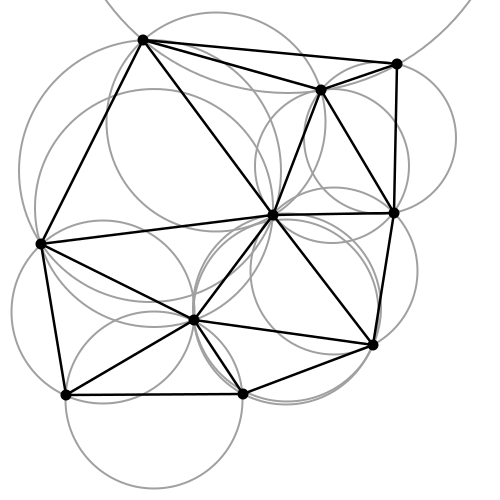
\includegraphics[width=0.8\textwidth]{images/3_0.png}
	\end{center}
	\caption{Пример триангуляции Делоне}
	\label{pic:delaunay_triangulation}
\end{wrapfigure} 
\par
Неравномерной сеткой называется модель описания поверхности в виде множества отдельных точек $\{(x_0, y_0), ..., (x_{n-1}, y_{n-1})\}$, принадлежащих поверхности.
\par
Использование равномерной сетки не всегда будет давать качественный результат для поиска кратчайшего пути, поэтому необходимо опробовать алгоритмы поиска кратчайшего пути на неравномерной сетке. Наиболее универсальной является треугольная сетка, так как не возникает проблем построения треугольников по каким-либо имеющимся данным.
\par
Для её построения воспользуемся триангуляцией Делоне.
Триангуляция Делоне --- триангуляция для заданного множества точек S на плоскости, при которой для любого треугольника все точки из S за исключением точек, являющихся его вершинами, лежат вне окружности, описанной вокруг треугольника \cite{Delaunay}. 

\subsection*{\Large{3.2 Получение точек }}
\addcontentsline{toc}{subsection} {3.2 Получение точек}
\hskip 12 mm
За получение координат точек сетки отвечает метод, логика работы которого реализована следующим образом. На вход ему подаются координаты точек, отвечающих за границы прямоугольника, лежащего на земной поверхности, внутри которого мы хотим найти кратчайший путь между парой точек. Результат работы метода зависит от двух параметров, которые задаются извне:
$d$ - размер сетки, $\gamma$ - коэффициент случайного смещения точек упорядоченной сетки.
\par
Далее мы вычисляем длины сторон заданного прямоугольника и делим их на размер сетки $d$, тем самым получая количество точек $n$ и $m$, лежащих на каждой из сторон прямоугольника. После этого получаем набор точек с одинаковыми интервалами между ними, для каждой из сторон, таким образом получаем упорядоченную сетку. Но упорядоченная сетка не всегда хороша для поиска кратчайшего пути, поэтому за внесения смещения в финальный набор точек отвечает параметр $\gamma \in [0.0,2.0]$. Таким образом из прямоугольной упорядоченной сетки мы получаем неупорядоченную. Итоговый набор точек получается по следующей формуле:\\
\centerline{ $\left\{\begin{matrix}
	\overrightarrow{M_x} = \overrightarrow{x} + \gamma \Delta_x \overrightarrow{\xi} \\ 
	\overrightarrow{M_y} = \overrightarrow{y} + \gamma \Delta_y \overrightarrow{\xi}
	\end{matrix}\right.$,} \\
где $\overrightarrow{M_x}, \overrightarrow{M_y}$ - итоговые координаты точек;\\
$\overrightarrow{x}, \overrightarrow{y}$ - координаты точек упорядоченной сетки;\\
$\Delta_x, \Delta_y$ расстояние между соседними точками упорядоченной сетки по $x$ и $y$;\\
$\xi \in [-0.5, 0.5]$ - значение случайной величины.
\par
Визуальные отличия сеток с различными значениями параметра $\gamma$ представлены в Приложение А.

\subsection*{\Large{3.3 Выбор модельных карт местности}}
\addcontentsline{toc}{subsection} {3.3 Выбор модельных карт местности}
\hskip 12 mm
Для тестирования работы программы были выбраны следующие модельные карты местности:
\begin{enumerate}
	\item {
		Квадрат размером [1.0 x 1.0] градусов. Ищем путь между точками, лежащими в противоположных углах квадрата. Эталонная длина пути: \mbox{157252.787 м.} Эта карта служит, как простейший случай для проверки правильности работы алгоритма поиска пути.
		\begin{figure}[H]
		    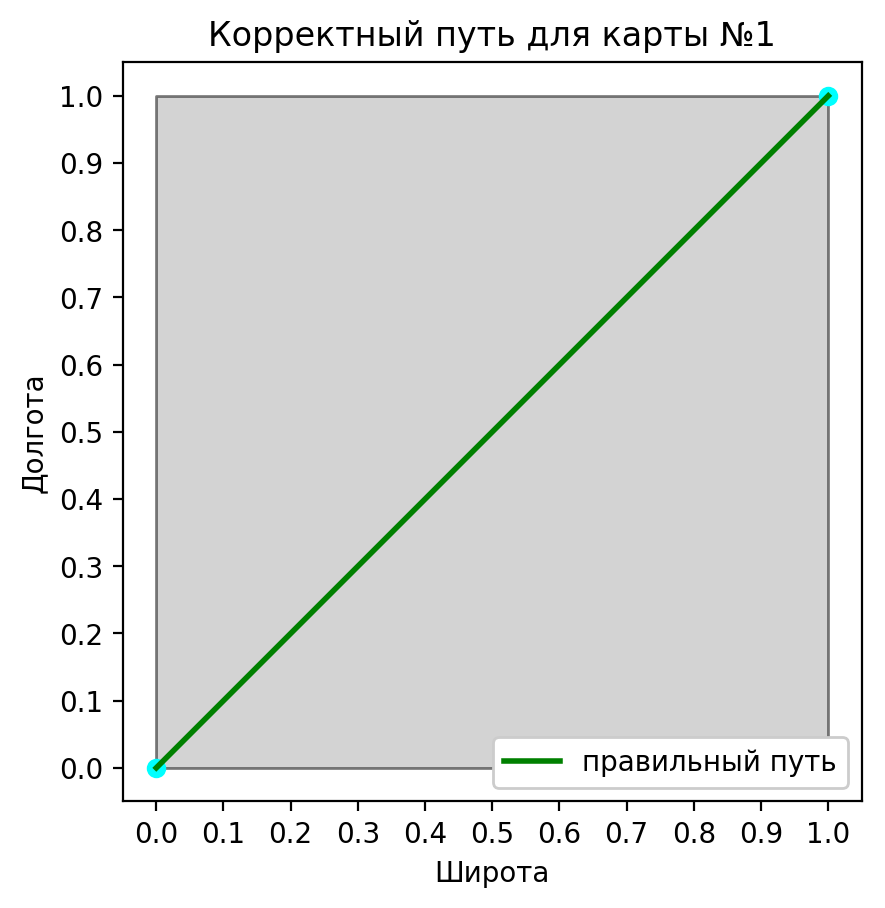
\includegraphics[width=0.5\textwidth]{images/3_1.png}
			\caption{Корректный путь для первой карты}
			\label{pic:correct_first}
		\end{figure}
	\vspace{2mm}
	}
	\item {
		Прямоугольник размером [1.0 x 0.1] градусов. Ищем путь между точками, лежащими в противоположных углах прямоугольника. Эталонная длина пути: 111751.882 м. Данная карта показывает некорректное построение пути, если использовать упорядоченную сетку.
		\begin{figure}[H]
			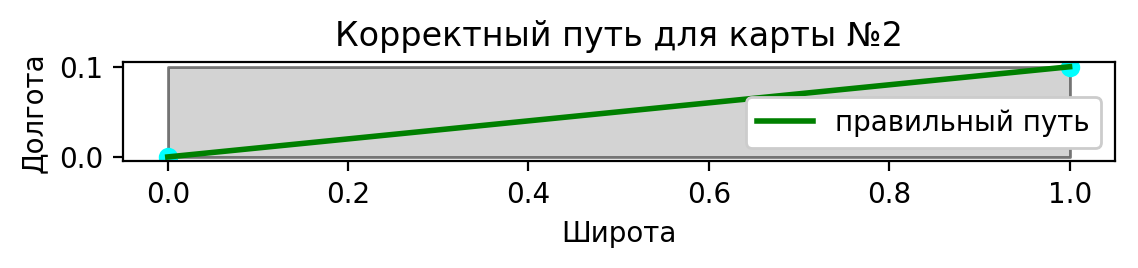
\includegraphics[width=0.9\textwidth]{images/3_2.png}
			\caption{Корректный путь для второй карты}
			\label{pic:correct_second}
		\end{figure}
	\vspace{2mm}
	}
	\item {
		Квадрат размером [0.9 x 0.9] градусов, который содержит в себе три зоны. Ищем путь между точками, лежащими в противоположных углах квадрата. Эталонный вес пути: 181256.383. Данная карта содержит в себе три зоны с разной стоимостью.
		\begin{figure}[H]
			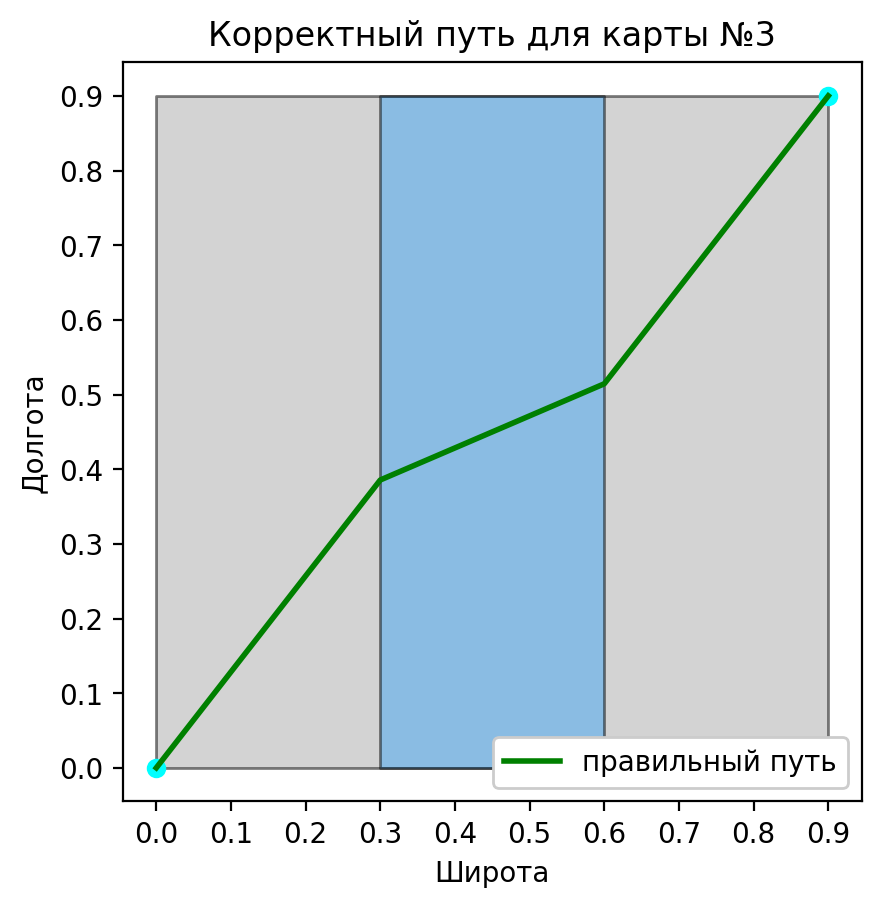
\includegraphics[width=0.5\textwidth]{images/3_3.png}
			\caption{Корректный путь для третьей карты}
			\label{pic:correct_third}
		\end{figure}
	\vspace{2mm}
	}
	\item { 
		Квадрат размером [1.0 x 1.0] градусов, содержащий в себе вписанную в себя сферу. Ищем путь между противоположными углами квадрата. Эталонная длина: 198523.065 м. Добавлен рельеф на карту.
		\begin{figure}[H]
			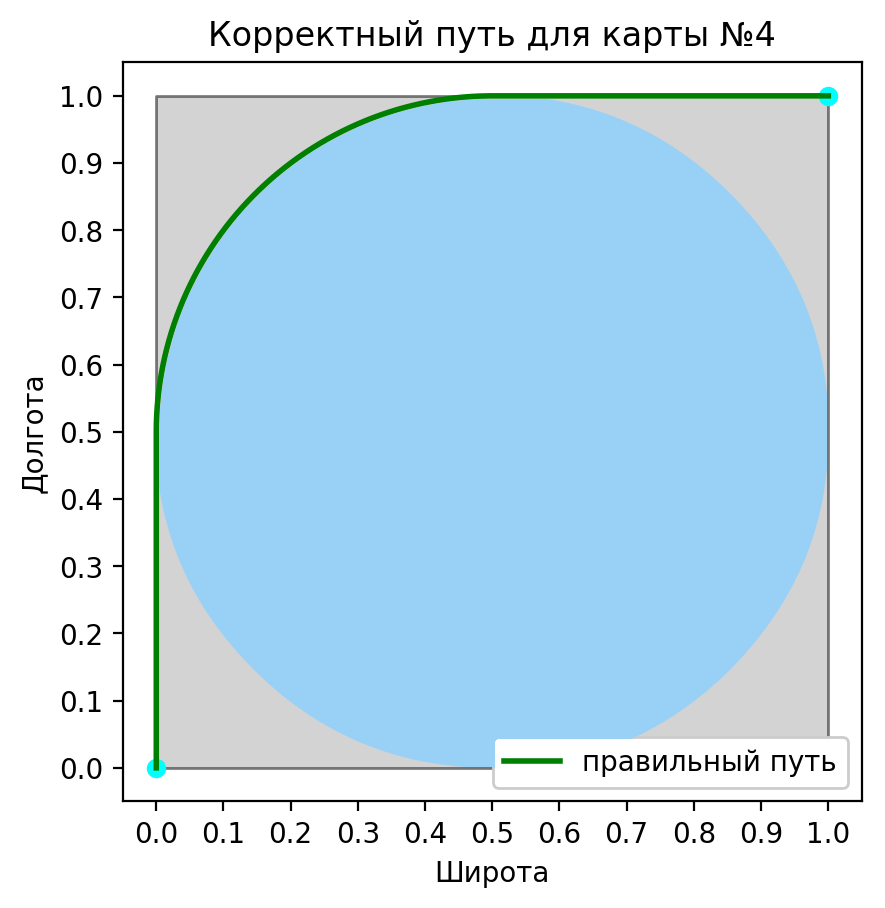
\includegraphics[width=0.5\textwidth]{images/3_4.png}
			\caption{Один из корректных путей для четвертой карты}
			\label{pic:correct_fourth}
		\end{figure}
	\vspace{2mm}
		}
	\item {
		Квадрат размером [1.0 x 1.0] градусов, содержащий в себе вписанную в себя сферу. Ищем путь между противоположными точками на сфере. Эталонная длина: 174668.365 м. Карта совпадает с предыдущей, но здесь мы ищем путь между противоположными точками, лежащими на сфере.
		\begin{figure}[H]
			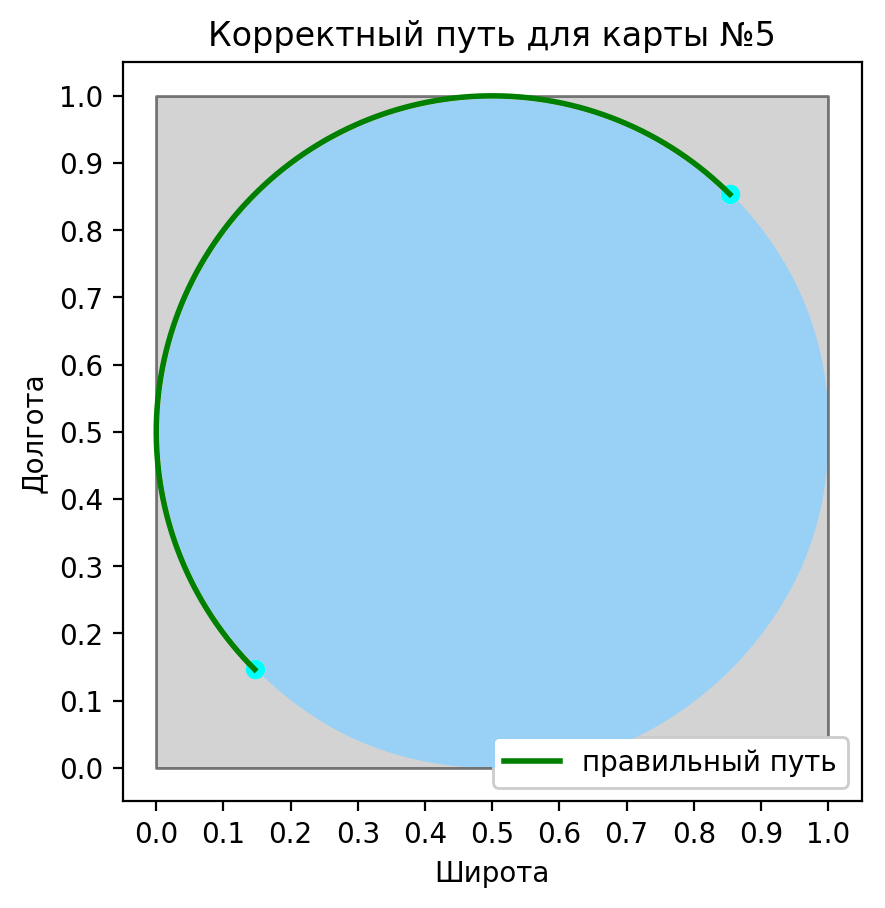
\includegraphics[width=0.5\textwidth]{images/3_5.png}
			\caption{Один из корректных путей для пятой карты}
			\label{pic:correct_fifth}
		\end{figure}
	\vspace{2mm}
		}
\end{enumerate}

\par
\subsection*{\Large{3.4 Проведение измерений}}
\addcontentsline{toc}{subsection} {3.4 Проведение измерений}
\hskip 12 mm
Основная задача данной главы заключалась в исследовании, насколько выбор параметров для построения сетки влияет на точность пути. Для оценки этих измерений мы использовали относительную ошибку пути, вычисляемую по формуле:\\
\centerline{$error = \frac{|Length_{correct} - Length_{path}|}{Length_{correct}} \cdot 100$,\\}
где $Length_{correct}$ - эталонная длина пути, найденная аналитически;\\
$Length_{path}$ - длина пути, полученная в результате работы алгоритма.

Путь представляет собой набор вершин $P: \forall \vec{p} \in P, \vec{p} = 
\bigl(\begin{smallmatrix}
x\\ 
y\\ 
h
\end{smallmatrix}\bigr)$, для которого длина вычисляется по формуле:\\
\centerline{$length =  \sum_{i = 0}^{n - 1}\rho_T(p_i, p_{i+1})$,} \\
где $\rho_T(p_i, p_j) = \sqrt{\rho_S(x_i, y_i; x_j, y_j)^2 + (h_i - h_j)^2}$,
$\rho_S$ - геодезическое расстояние между точками на сфере. 

Измерения проводились следующим образом: для каждой из карт мы
перебирали значения $\gamma$ на отрезке $[0.0, 2.0]$ с шагом 0.2 и различные размеры
сетки. Для начала требовалось определить, какая верхняя граница размеров
сетки будет давать достаточно низкое значение ошибки. Для этого была
использована первая карта. На отрезке [75, 27800] был выбран 51 различный
размер $d$. В итоге был получен следующий график зависимости ошибки пути
от значений $\gamma$ и $d$ (см. рис. \ref{pic:error_75_27800}):
\begin{figure}[H]
	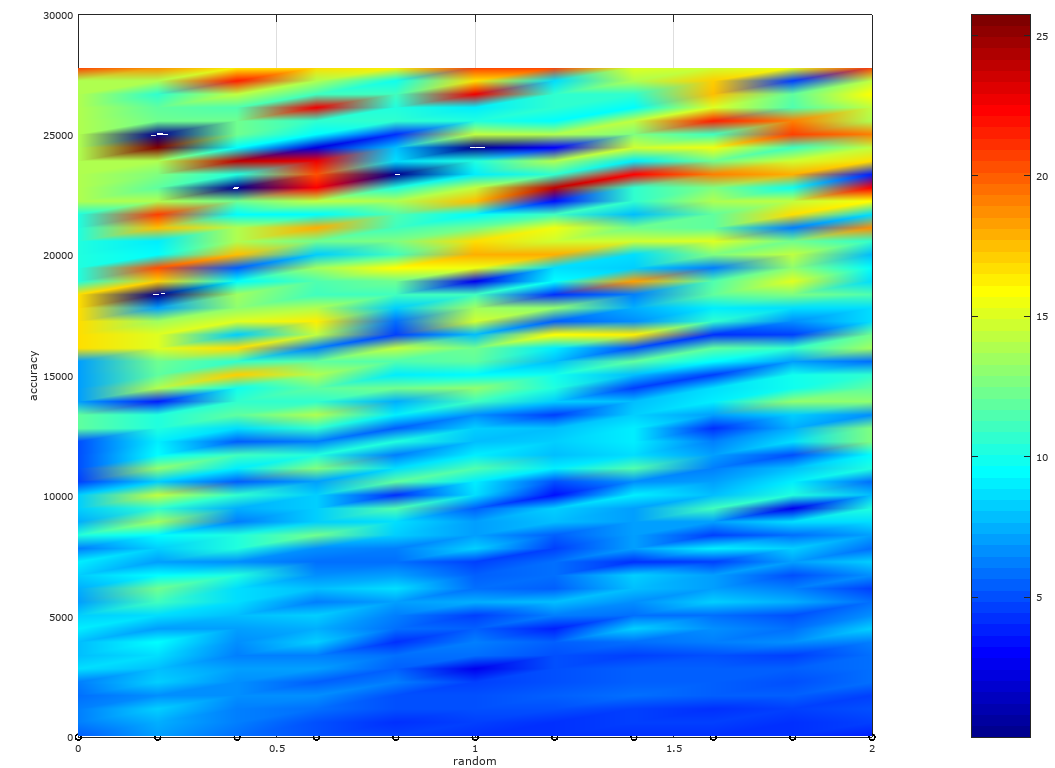
\includegraphics[width=\textwidth]{images/3_6.png}
	\caption{График значений размера ошибки на [75, 27800]}
	\label{pic:error_75_27800}
\end{figure}
\vspace{2mm}
Исходя из этого графика, видно, что достаточно низкие величины
ошибок, которые стабильны на всем диапазоне случайной величины,
достигаются, если размер сетки $d$ не превышает 5000 м, что составляет чуть
менее 5\% от размеров стороны квадрата. Найдем еще более точную правую
границу. Рассмотрим график значений ошибки для значений $d$ на отрезке [50, 5000] (см.
рис. \ref{pic:error_50_5000}):
\begin{figure}[H]
	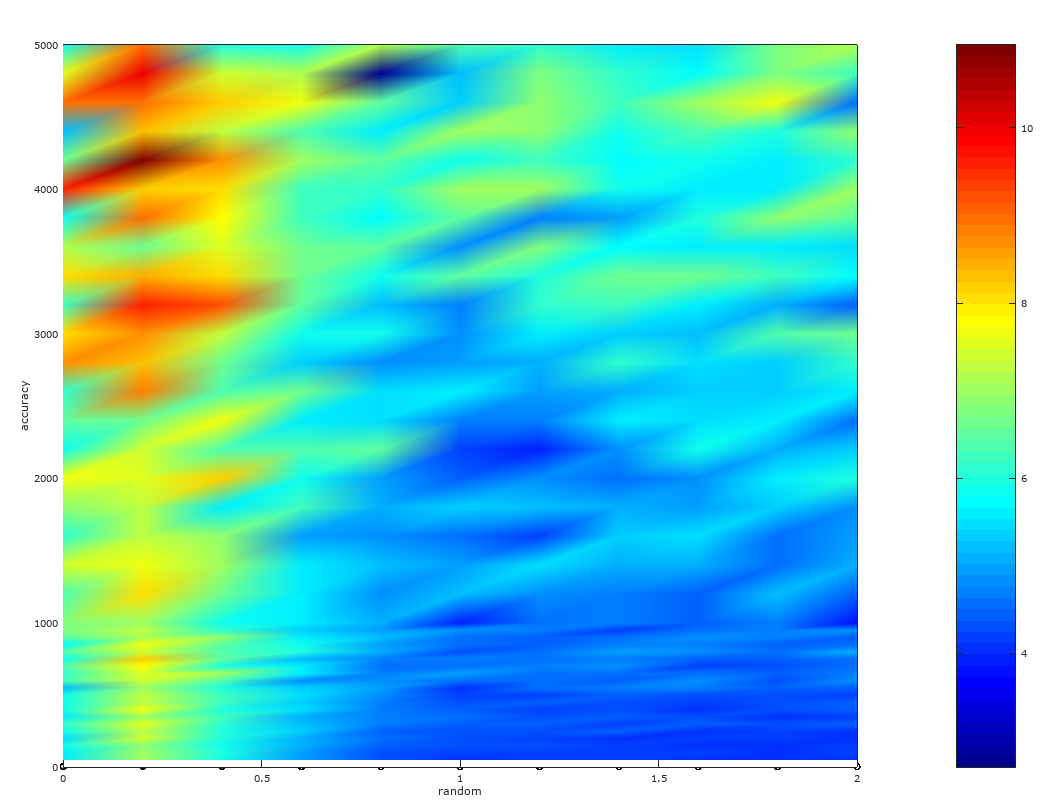
\includegraphics[width=\textwidth]{images/3_7.png}
	\caption{График значений размера ошибки на [50, 5000]}
	\label{pic:error_50_5000}
\end{figure}
\vspace{2mm}
Отсюда мы видим, что наиболее качественные результаты получаются
на отрезке [50, 500], что в относительных величинах, составляет от 0.05\% до
0.5\% относительно стороны квадрата. В дальнейшем мы будем искать
кратчайшие пути, используя только этот диапазон.\\
Определив диапазон значений, перейдем непосредственно к результатам
поиска кратчайшего пути и некоторым особенностям, связанным с этим.
\begin{itemize}
\item{
Значение $\gamma$ = 0.2 оказалось наихудшим для первой карты, что видно на
рисунке(см. рис. \ref{pic:error_first}):
\begin{figure}[H]
	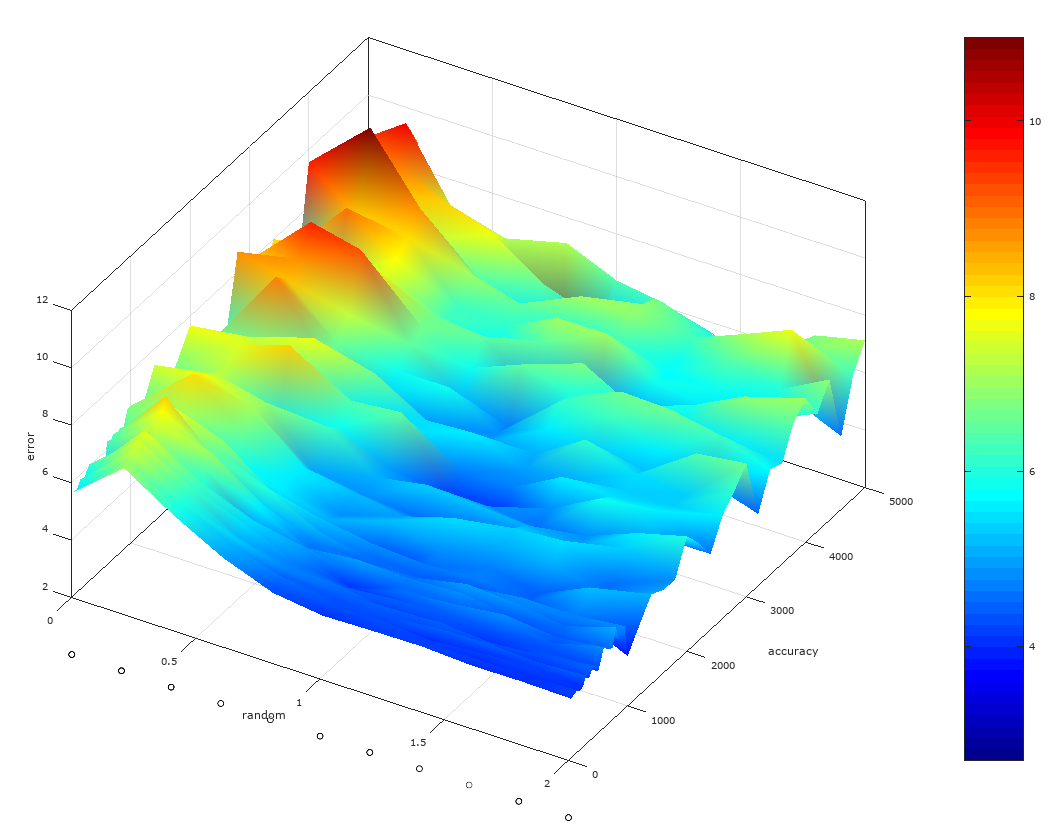
\includegraphics[width=\textwidth]{images/3_8.png}
	\caption{Значения ошибки для первой карты}
	\label{pic:error_first}
\end{figure}
\vspace{2mm}
Была замечена закономерность, что при $\gamma < 0.5$ были получены
наибольшие величины ошибки для всех карт. Но наиболее гладкий
путь для второй карты получается, как раз, при значении $\gamma = 0.2$.
Однако, величина ошибки от этого все равно не стала минимальной.
Это явление можно увидеть на рисунках ниже.
\begin{figure}[H]
	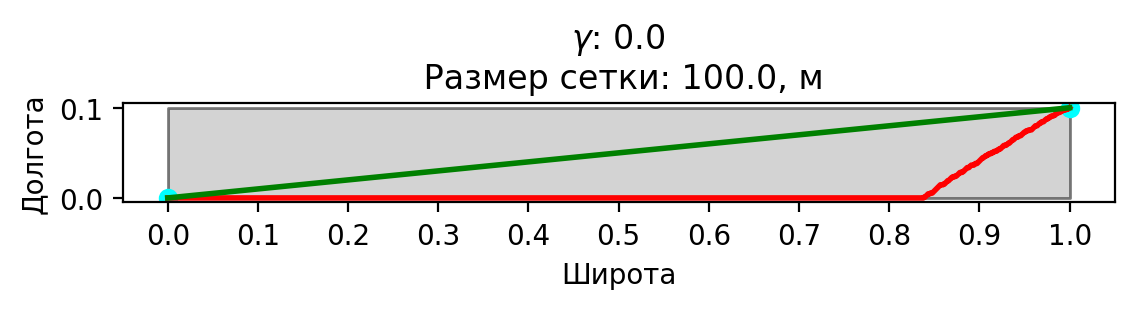
\includegraphics[width=0.9\textwidth]{images/3_9.png}
	\caption{Путь для второй карты при $\gamma = 0.0$}
	\label{pic:path_2_1}
\end{figure}
\vspace{2mm}
\begin{figure}[H]
	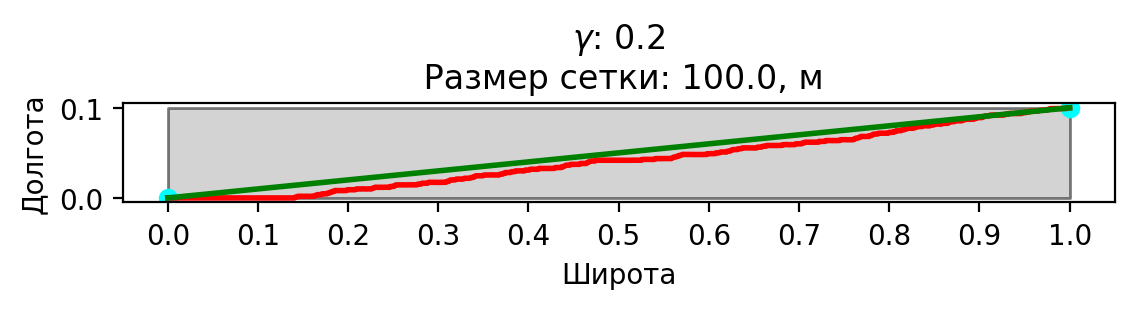
\includegraphics[width=0.9\textwidth]{images/3_10.png}
	\caption{Путь для второй карты при $\gamma = 0.2$}
	\label{pic:path_2_2}
\end{figure}
\vspace{2mm}
}
\item {
	Проблема правильности вычисления длины пути на карте с рельефом.
	При построении пути на карте со сферой появились отрицательные
	значения ошибки длины пути. Данная проблема была связана со
	следующим явлением (см. рис. \ref{pic:short_length_problem_1}):
	\begin{figure}[H]
		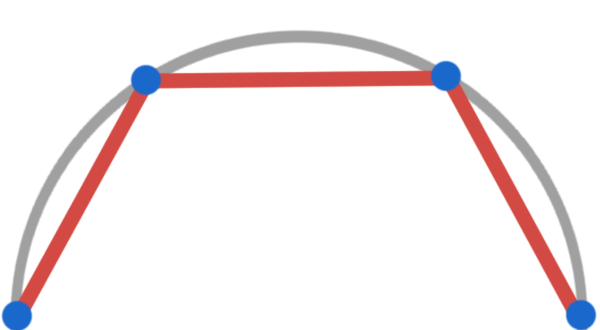
\includegraphics[width=0.4\textwidth]{images/3_11.png}
		\caption{Проблема меньшей длины пути}
		\label{pic:short_length_problem_1}
	\end{figure}
	\vspace{2mm}
	Длина дуги окружности будет всегда больше, чем длина
	пути на многоугольнике, который аппроксимирует эту окружность.
	Аналогичная ситуация возникает на абсолютно любой карте с
	использованием рельефа. Поэтому для карт с рельефом важно
	разбивать, полученный путь на более мелкие части, чтобы правильно
	вычислять длину пути. 
}	
\end{itemize}

Для сбора статистики для каждой карты были проверены размеры сетки
$d$, лежащие в отрезке [100, 500] с шагом в 50 м и значения $\gamma$ на отрезке [0.0, 2.0] с шагом 0.2. После получения наборов вершин, представляющих собой
пути, к ним был применен алгоритм сглаживания методом скользящего
среднего с разным размером окна $w$, который составлял от 3 вершин до трети
количества вершин длины пути. Сглаживание пути на карте с рельефом
проводилось на детализированном пути (см. рис. \ref{pic:detailed_path}) для корректного
вычисления длины пути: $d$ – текущий размер сетки, $m$ - минимальный размер
сетки.
\begin{figure}[H]
	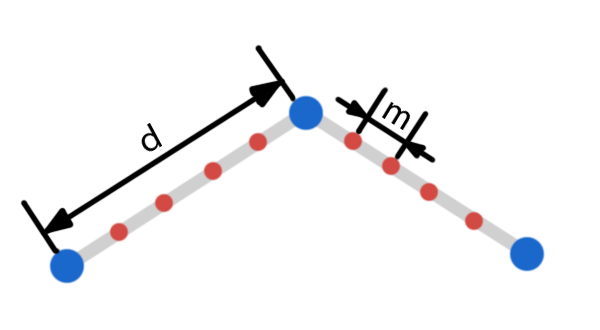
\includegraphics[width=0.6\textwidth]{images/3_13.png}
	\caption{Детализированный путь}
	\label{pic:detailed_path}
\end{figure}
\vspace{2mm}
\subsection*{\Large{3.5 Анализ результатов}}
\addcontentsline{toc}{subsection} {3.5 Анализ результатов}
\hskip 12 mm
По завершении работы были получены следующие итоговые таблицы с результатами.
\begin{table}[H]
	\centering
	\caption{Наилучшие результаты для начального пути}
	\label{tabular:best_results_1}
	\begin{tabular}{|c|c|c|c|c|}
		\hline
		\textbf{Карта}     & \textbf{Ошибкаб \%} & \textbf{$d$, м} & \textbf{$\gamma$} & \textbf{$w$}   \\ \hline
		1 &    3.973  &  500 м & 2.0 & None  \\ \hline
		2 &  2.029 & 500 м & 1.4 & None \\ \hline
		3 &  3.731 & 300 м & 1.2 & None \\ \hline
		4 & 1.734 & 100 м & 2.0 & None \\ \hline
		5 & 1.600 & 300 м  & 1.8 & None \\ \hline
	\end{tabular}
	
\end{table}
\vspace{2mm}
\par
\begin{table}[H]
	\centering
	\caption{Наилучшие результаты для сглаженного пути}
	\label{tabular:best_results_2}
	\begin{tabular}{|c|c|c|c|c|}
		\hline
		\textbf{Карта}     & \textbf{Ошибка, \%}  & \textbf{$d$, м} & \textbf{$\gamma$} & \textbf{$w$}   \\ \hline
		1 & 0.018 & 150 м & 0.8 & 322 \\ \hline
		2 & 0.055 & 100 м & 0.2 & 370 \\ \hline
		3 & 0.011 & 500 м & 0.8 & 29 \\ \hline
		4 & 0.099 & 100 м & 0.6 & 530 \\ \hline
		5 & 0.025 & 150 м & 0.6 & 283 \\ \hline
	\end{tabular}
\end{table}
\vspace{2mm}
\par
Если мы хотим получить изначальный путь достаточно высокого
качества, то значение $\gamma$ должно лежать в отрезке [1.4, 1.8]. Если мы потом собираемся
применять алгоритмы сглаживания к построенному пути, то значение $\gamma$
должно лежать в отрезке [0.6, 0.8]. Сглаживание пути принесло улучшение результата во
всех рассмотренных случаях. Размер окна сглаживания $w$ в среднем не превосходит 15-20\%
от общего количества вершин пути. Поэтому как правое ограничение окна
сглаживания можно установить на уровне 5-9\% от количества вершин пути.
\par
При значении $\gamma$ равном 0.0 или 0.2 были получены пути с наибольшим
значением ошибки, как для обычного пути, так и для сглаженного.
\par
Временная сложность данного алгоритма является квадратичной(так как основную часть времени
работы алгоритма составляет добавление элементов сетки в граф). Ниже представлена
таблица зависимости времени работы алгоритма к размеру сетки для первой карты (см. табл. \ref{tabular:accuracy_time_1}):
\begin{table}[H]
	\centering
	\caption{Время работы алгоритма в зависимости от размера сетки}
	\label{tabular:accuracy_time_1}
\begin{tabular}{|c|c|c|c|c|c|c|c|c|c|c|}
		\hline
		50 & 100 &	150 &	200 &	250 &	300 &	350 &	400 &	450 &	500 &	$d$, м \\ \hline
		353	& 82 &	36 &	20	& 12.5 &	8.75 &	6.7 &	4.85 &	3.5	& 2.93 &	$t$, сек \\ \hline
\end{tabular}
\end{table}
\vspace{2mm}
\par
Эти данные позволяют нам сделать вывод о том, что достаточно
высокую точность пути можно получить и не используя очень мелкую сетку.
И можно достигать вполне эффективных результатов и с $d$ = 300 м.
